问题四需要解决的核心识别问题，是将前三问给出的 Loss 机制与现实模型的 Benchmark 表现统一到可比较的能力尺度。前三问依次刻画数据质量与领域配比、广义标度关系及算力约束下的最优资源配置，由此形成从预算到最优损失的机制映射 $L^*(C)$；现实样本则提供综合能力前沿 $F_t$ 和训练算力前沿 $C_t$。对两类前沿分别实施时间回归，既不能从回归系数中识别规模效应，也无法构造算力增速放缓的结构反事实。为此，本文引入 Loss--Benchmark 桥接函数 $H$ 作为观测映射，并建立统一状态方程
\begin{equation}
F_t-F_{t_0}
=\underbrace{H[L^*(C_t)]-H[L^*(C_{t_0})]}_{\text{规模机制项}}
+\underbrace{T_t}_{\text{非规模技术综合项}}
\label{eq:q4-state}
\end{equation}
其中，$T_t$ 表示前三问规模机制不能解释的锚定残差，综合反映架构、优化方法、数据工程、后训练及未观测因素，不再将其归属于某项单一技术。图~\ref{fig:q4-framework}给出从前三问机制输出到能力度量、桥接、贡献分解与预测的完整链路。历史分解与未来预测共用式~\eqref{eq:q4-state}，桥接误差和支持边界亦沿同一链路传播。后续分析依次识别 $F_t$、估计 $H$、构造 $B(C)=H[L^*(C)]$，并据此分解历史增长与推演未来前沿。

\begin{figure}[htbp]
    \centering
    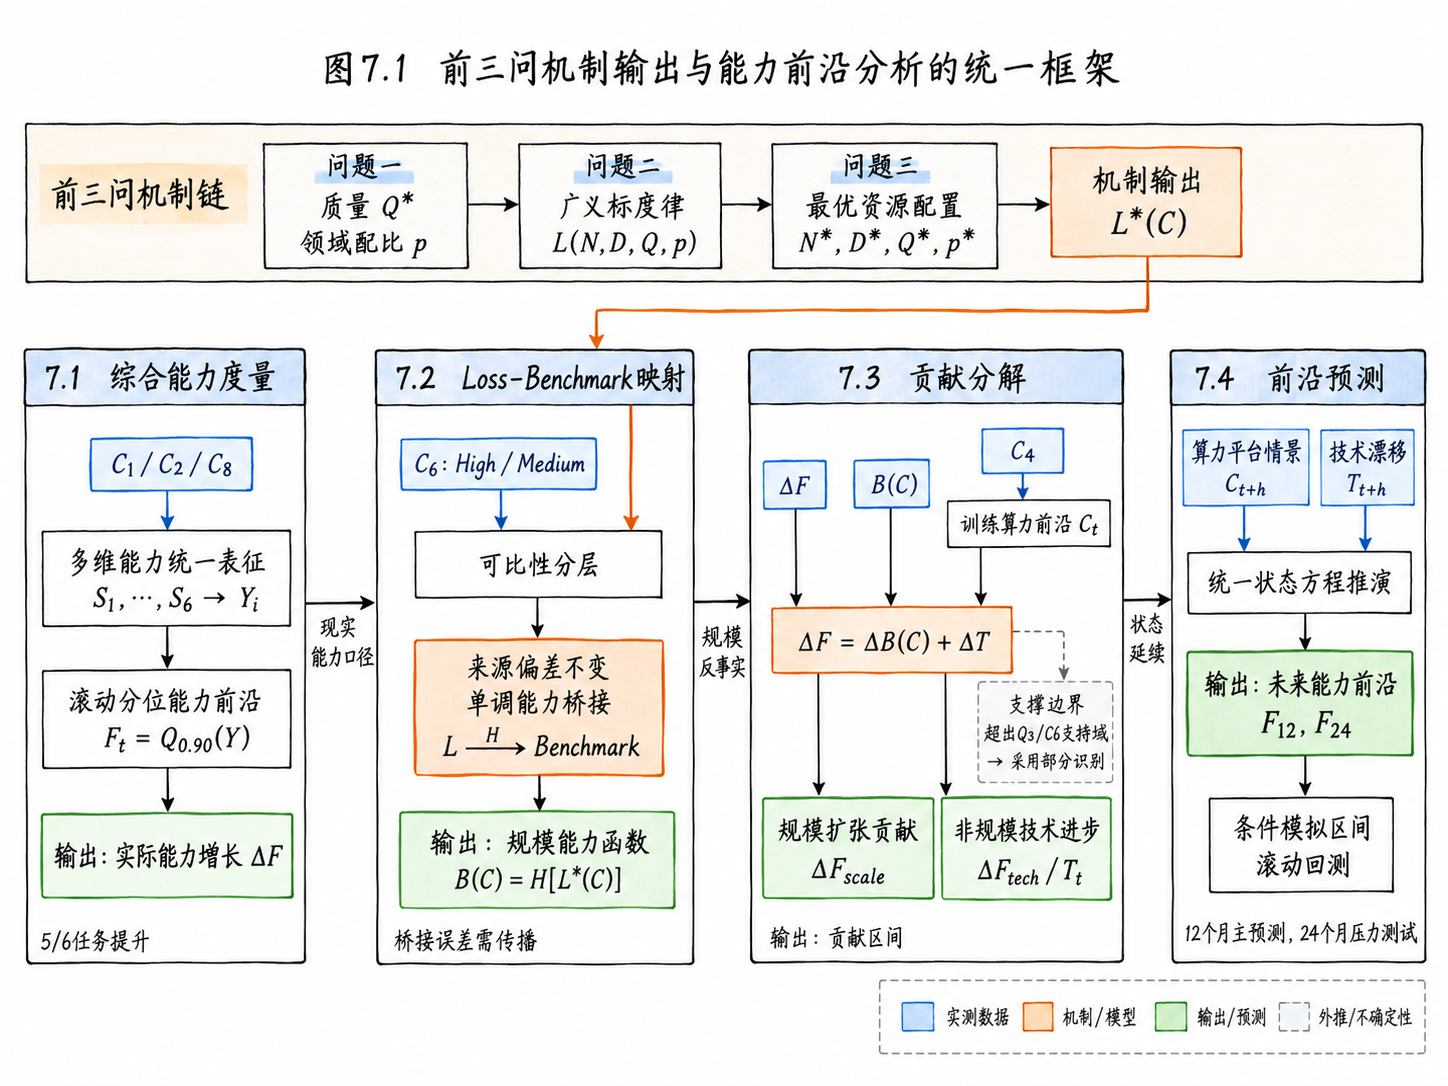
\includegraphics[width=0.90\textwidth,height=0.35\textheight,keepaspectratio,trim=0 0 0 3.05cm,clip]{figures/fig7_1.png}
    \caption{前三问机制输出与能力前沿分析的统一框架}
    \label{fig:q4-framework}
\end{figure}

\subsection{开放权重模型综合能力度量}

本节首先确定现实能力的观测状态及其可靠性，再将该状态传递给后续桥接与贡献分解。具体而言，先建立可比较的综合能力坐标，再以滚动高分位提取时间前沿，并从任务维度、指标口径和模型族依赖三个层面检验其稳健性。

\subsubsection{开放权重模型的多维能力统一表征}

能力口径首先满足“对象可比、时间可追溯、任务完整”。主样本限定为开放权重的 chat 或领域微调模型，以 Open LLM Leaderboard 的 Submission Date 作为能力出现时间，并要求 IFEval、BBH、MATH Lvl 5、GPQA、MUSR、MMLU-PRO 六项得分完整。pretrained 模型只作为类型对照；许可证字段另按 Apache、MIT、BSD、CC-BY、OpenRAIL 及可研究模型族许可证构造严格子样本，但该文本规则不解释为法律合规认证。各数据源的角色和时间合同见表~\ref{tab:q4-data-contract}。

\begin{table}[htbp]
\caption{问题四的数据口径、时间合同与证据角色}
\label{tab:q4-data-contract}
\CompactTableSetup
\begin{tabularx}{0.92\textwidth}{@{}C{1.15cm}L C{2.00cm}C{1.25cm}C{1.40cm}@{}}
\toprule
数据 & 主筛选与变量 & 时间轴 & 样本量 & 证据角色\\
\midrule
C1/C2 & 开放权重、六项完整、chat/finetuned & Submission Date & 231 & 能力主前沿\\
C8 & 最新可解析快照、六项任务得分 & 评测时间 & 1854 & 逐任务诊断\\
C4 & Language、LM/QA、可信 reported compute & Publication date & 326 & 算力主前沿\\
C6 & High 与 Medium 分层保留 & 不进入时间轴 & 7+68 & Loss--能力桥接\\
Q3 & 主情景、context 4096、三档预算 & 算力预算 & 3个锚点 & 规模机制\\
\bottomrule
\end{tabularx}
\TableNote{注：C8 共审计1860个唯一模型，其中1854个六维完整；C4 的 $6ND$ 估计仅进入敏感性分析。}
\end{table}

六项指标分别刻画指令遵循、综合推理、数学、研究生层次问答、多步软推理与专业知识。为避免由样本方差替研究目标赋权，主分析采用等权均值 $Y_i=\frac{1}{6}\sum_{k=1}^{6}S_{ik}$，使结果仍保持0--100分的直观解释。等权并不意味着六项完全同质：其作用是构造稳定、透明的共同能力坐标，PCA和任务内标准化均值只用于检验该坐标是否被单项量纲支配。

六项原始得分的 Cronbach $\alpha=0.826$，达到较好的内部一致性\cite{cronbach1951}；标准化 PCA 的第一主成分解释率为65.1\%，等权得分与第一主成分、任务内标准化均值的相关系数分别为0.960和0.977。三种能力口径的前沿净变化方向均为正，说明等权指标既保留可解释性，也未偏离数据中的主要共同变化方向。

\subsubsection{基于滚动分位的能力前沿构建}

单个榜首模型易受偶然提交、测试噪声和同族微调影响，月均值又会被大量普通提交拖动。本文在每个月末向前取三个月，以综合能力的90\%分位定义开放权重能力前沿：
\begin{equation}
F_t=Q_{0.90}\!\left\{Y_i\,\middle|\,t-3\text{月}<t_i\le t\right\}.
\label{eq:q4-frontier}
\end{equation}
该定义衡量当期可稳定达到的高能力区域，而非单一最高值。主样本在2024年6月至2025年3月形成10个有效月度点，前沿从30.754升至39.062，观测净增长为8.307分。图~\ref{fig:q4-capability}a同时保留全部模型散点和2/3/4个月、Q90/Q95六种方案的包络，主曲线始终处于敏感性范围内。

\begin{figure}[htbp]
    \centering
    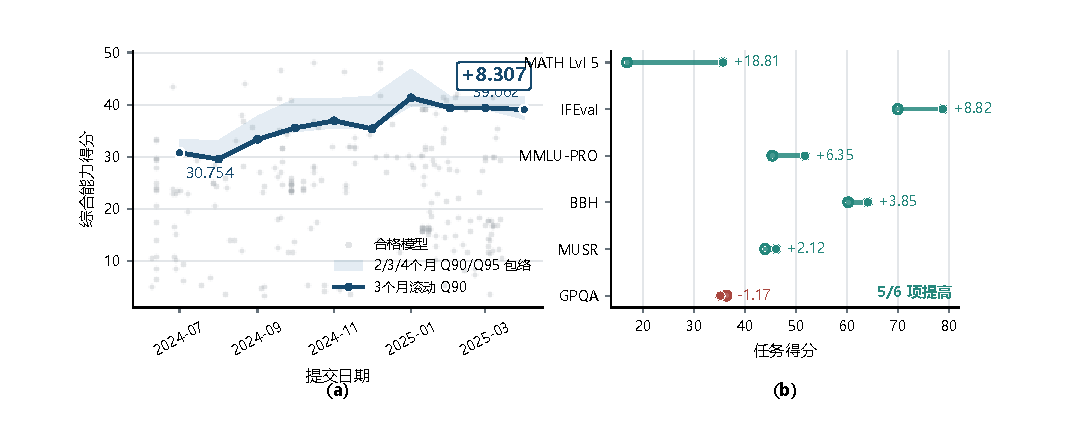
\includegraphics[width=0.92\textwidth,height=0.27\textheight,keepaspectratio]{figures/fig7_2_capability_frontier.pdf}
    \caption{开放权重模型综合能力前沿与逐任务演进广度}
    \label{fig:q4-capability}
\end{figure}

\subsubsection{能力前沿的逐任务与多口径检验}

图~\ref{fig:q4-capability}b显示，首末窗口的六项任务中有五项提高：MATH Lvl 5、IFEval、MMLU-PRO、BBH、MUSR 分别增加18.807、8.825、6.355、3.853和2.116分，GPQA下降1.174分。月度任务改善广度的中位数为4/6。因此，8.307分增长具有较广的任务基础，但并不表明各维能力同步改善。C8中MATH的154个精确零值保留为困难任务的有效得分；未发现重复模型、重复结果文件或集中性快照故障。

进一步控制重复提交后，按基础架构正则识别模型族，无法识别时退回 Hugging Face 组织名；每个模型族每月仅保留最高能力模型，54个“族--月”单元的前沿仍增长8.238分。按“月份$\times$模型族”进行2000次块 Bootstrap，净增长为正的比例为93.8\%，中位数6.804分，2.5\%--97.5\%分位为$[-2.201,15.732]$。该结果排除了热门模型族重复提交对主增长的完全解释，但仍保留6.2\%重采样不增长这一不确定性。类型对照中，pretrained 前沿提高5.731分，小于 chat/finetuned 的8.307分，提示后训练可能参与能力推进；由于两类样本构成不同，本文不把差值解释为后训练的因果贡献。

\begin{table}[htbp]
\caption{综合能力指标与能力前沿的多层稳健性检验}
\label{tab:q4-capability-validation}
\CompactTableSetup
\begin{tabularx}{0.92\textwidth}{@{}L L C{2.40cm}Y@{}}
\toprule
检验层次 & 统计量或对照 & 结果 & 证据含义\\
\midrule
内部一致性 & Cronbach $\alpha$ & 0.826 & 六项任务具有较好可合成性\\
共同因子 & 第一主成分解释率 & 65.1\% & 存在占主导的共同能力方向\\
口径一致性 & 等权与PCA/标准化均值相关 & 0.960/0.977 & 结论不受单一量纲支配\\
前沿口径 & 等权、PCA、标准化均值 & 净变化均为正 & 上升方向不依赖合成方法\\
模型族平衡 & 每族每月仅留最优模型 & $+8.238$分 & 重复提交不能解释主增长\\
相关性重采样 & 族--月块Bootstrap 2000次 & 93.8\%为正 & 方向稳健，但保留6.2\%反例\\
模型类型 & pretrained与chat/finetuned & 5.731/8.307分 & 异质性提示，不作因果归因\\
\bottomrule
\end{tabularx}
\TableNote[0.92\textwidth]{注：主模型始终采用等权能力口径；PCA、标准化均值及类型拆分仅用于稳健性检验。}
\end{table}

表~\ref{tab:q4-capability-validation}依次检验指标的可合成性、方向一致性、重复提交影响及模型类型异质性。由此得到统一状态方程中的观测状态 $F_t$；后续以8.307分作为历史增长事实，并将模型族依赖纳入Bootstrap。下一节进一步估计连接 Loss 与该能力状态的观测映射 $H$。

\subsection{Loss--Benchmark能力映射}

能力前沿给出了现实模型的观测尺度，但尚未回答前三问的最优损失如何进入该尺度。本节利用分层桥接样本估计 $H$，重点处理来源水平差异、单调机制约束及小样本验证误差，并将桥接结果作为规模能力函数的唯一观测接口。

\subsubsection{桥接样本的可比性分层}

前三问输出的是验证 Loss，式~\eqref{eq:q4-state}左侧却是 Benchmark 得分，两者不能直接相减。C6桥接样本共75条，其中7条 High 样本具有较强同协议可比性且均来自 Pythia，68条 Medium 样本覆盖更多模型族，但验证集、训练阶段或 Loss 定义存在差异。若将两层数据直接混合，来源的绝对水平差会被误当成能力响应；若只用7条 High 数据，又无法稳定辨识非线性形状。因此，本文让 High 提供水平锚点、Medium 提供形状信息，并显式分离来源截距与残差方差。

\subsubsection{来源偏差不变的单调能力桥接}

记 $I_i^{M}$ 为 Medium 指示变量，在 Loss 分位点 $\kappa_j$ 上构造铰链基函数，建立
\begin{equation}
Y_i=\alpha+\delta_M I_i^{M}
+\sum_{j=1}^{J}\beta_j(\kappa_j-L_i)_++\varepsilon_i,
\qquad \beta_j\ge0,\quad
\operatorname{Var}(\varepsilon_i)=\sigma_{g(i)}^2.
\label{eq:q4-bridge}
\end{equation}
非负约束保证 $H'(L)\le0$，即 Loss 降低不会预测出能力下降。High/Medium 分别估计残差尺度；考虑 High 仅7条，本文以5个先验自由度向总体方差作经验收缩，避免小样本方差过小而在加权拟合中占据不合理权重。相邻铰链系数的一阶差分惩罚控制局部斜率突变，惩罚强度由分层留出交叉验证确定为10。

估计的 Medium 来源截距为$\widehat\delta_M=11.824$分。绝对截距用于吸收跨来源 Loss 水平差异，而历史分解只使用同一桥接层内的差值
$H(L_1)-H(L_0)$，故固定来源偏差严格抵消。该“来源截距可变、能力差分不变”的设定适应了当前多源小样本条件，且无需假定不同来源具有统一的绝对 Loss 基准。图~\ref{fig:q4-bridge}a仅在C6观测范围$[1.65,2.84]$内绘制桥接曲线，灰色边缘不参与拟合外推。

\begin{figure}[htbp]
    \centering
    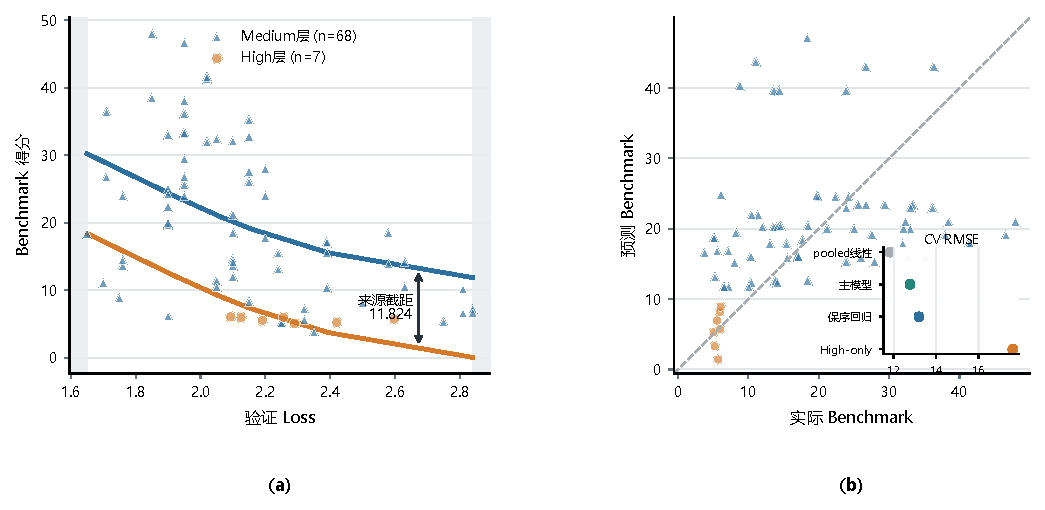
\includegraphics[width=0.92\textwidth,height=0.27\textheight,keepaspectratio]{figures/fig7_3_loss_benchmark_bridge.pdf}
    \caption{来源分层的Loss--Benchmark单调桥接与留出预测校准}
    \label{fig:q4-bridge}
\end{figure}

\subsubsection{分层留出验证与映射误差评估}

四类桥接统一采用“Medium留一模型族、High留一观测”的交叉验证，结果见表~\ref{tab:q4-bridge}. pooled线性模型的RMSE最低，主模型的MAE最低；主模型并非在所有误差指标上占优。本文仍选择来源校准单调样条，是因为贡献分解要求同时满足机制方向、来源偏差显式分离和差分不变性，不能只依据单一RMSE选模。

\begin{table}[htbp]
\caption{四类Loss--Benchmark桥接的统一留出验证}
\label{tab:q4-bridge}
\CompactTableSetup
\begin{tabularx}{0.84\textwidth}{@{}L C{1.25cm}C{1.65cm}Y@{}}
\toprule
桥接模型 & RMSE & MAE & 结构性质\\
\midrule
pooled线性 & \textbf{11.815} & 9.817 & 无来源校准、无形状约束\\
High-only线性 & 17.620 & 13.455 & 同协议但样本仅7条\\
无来源校准保序回归 & 13.190 & 10.318 & 单调但混合来源水平\\
来源校准单调样条（主模型） & 12.766 & \textbf{9.650} & 单调、分层方差、差分不变\\
\bottomrule
\end{tabularx}
\TableNote[0.84\textwidth]{注：四类模型均在同一75条留出预测上比较；加粗只表示对应误差指标的最小值。}
\end{table}

全样本 Loss 与能力的 Spearman 相关为$-0.549$，方向符合机制预期，但图~\ref{fig:q4-bridge}b显示绝对映射仍有明显离散。逐一删去7个Pythia观测后，末端斜率保持在$-24.61$至$-24.99$分/Loss，后续规模份额上界仅在8.431\%--8.561\%间变化，表明固定样本结论不由单个High观测主导。桥接误差仍是问题四的重要不确定性，须在后续条件模拟中完整传播。本节由此得到观测映射 $H$，下一节将其与问题三的 $L^*(C)$复合，形成规模能力函数 $B(C)$。

\subsection{规模扩张与非规模技术进步贡献分解}

在获得能力状态 $F_t$、桥接函数 $H$ 及问题三的最优损失曲线 $L^*(C)$ 后，本节考察历史能力增长中可由算力机制解释的部分。分析顺序为先构造与能力前沿同尺度的算力前沿，再形成 $B(C)=H[L^*(C)]$，最后在共同支持边界约束下给出贡献的部分识别集合。

\subsubsection{基于滚动分位的训练算力前沿构建}

为与能力前沿保持相同时间平滑尺度，训练算力前沿定义为开放权重Language域、language modeling或question answering任务中，Confident/Likely且真实报告训练FLOPs模型的三个月滚动Q90。共有617个模型满足基础元数据筛选，342个报告compute，其中326个进入可信主样本；72个仅能由$6ND$估计，203个缺失算力。主结果只使用reported compute，$6ND$仅构造敏感性曲线。

图~\ref{fig:q4-support}a显示，2023年6月至2024年6月的Theil--Sen斜率为每月$0.0812\ \log_{10}$FLOPs，2024年7月至2025年3月转为$-0.0429$。这表明2024年中跃升后进入平台/回落阶段；负的短窗口斜率不等于长期算力必然下降，故预测主情景将未来算力增速保守截为0。reported compute 与加入$6ND$后的前沿走势接近，结论不依赖估算值。

\begin{figure}[htbp]
    \centering
    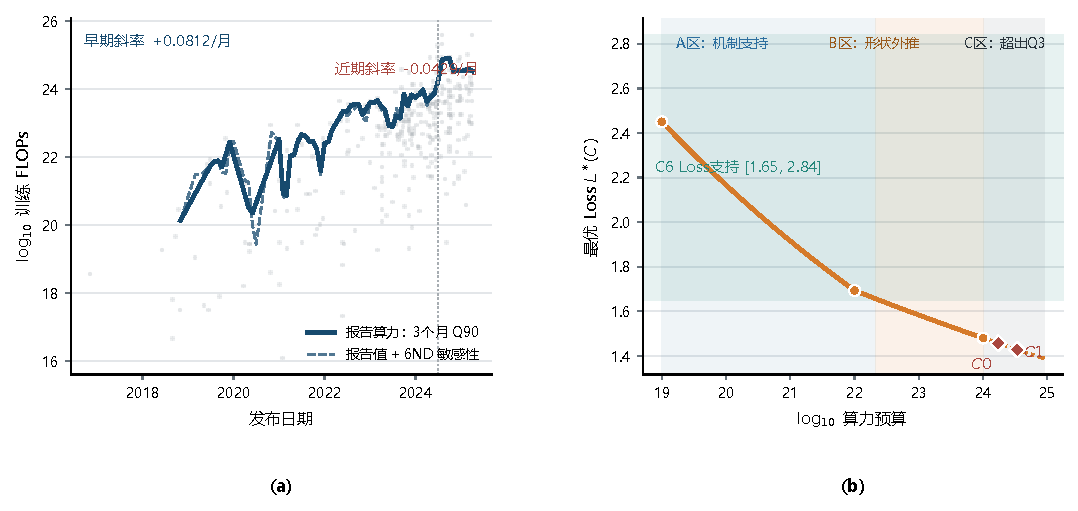
\includegraphics[width=0.92\textwidth,height=0.27\textheight,keepaspectratio]{figures/fig7_4_compute_and_support.pdf}
    \caption{训练算力演进与Q3--C6共同支持边界}
    \label{fig:q4-support}
\end{figure}

\subsubsection{机制锚定的规模能力反事实}

问题三主情景固定为context 4096、指数质量成本、ratio桥接与$\kappa=1$，在$10^{19},10^{22},10^{24}$ FLOPs三档预算下得到最优平均Loss 2.4500、1.6932、1.4803。本文仅在$\log C$--$\log L$空间对三锚点分段连接，形成继承前三问机制的$L^*(C)$，而不使用历史能力数据重新拟合“规模趋势”。由此定义规模能力函数
\begin{equation}
B(C)=H[L^*(C)],
\qquad
\Delta F_t=\Delta B(C_t)+T_t.
\label{eq:q4-mechanism}
\end{equation}
其中$B(C)$回答“在前三问配置机制与桥接关系保持不变时，仅改变算力预算应获得多少能力”。这一反事实直接连接问题三，而$T_t$只承接剩余变化，从而避免把时间回归系数直接命名为技术进步。

图~\ref{fig:q4-support}b将$L^*(C)$与C6 Loss范围叠加。Level A为较强机制支持区，Level B依赖响应形状延伸，$C>10^{24}$ FLOPs的Level C超出Q3预算。观测窗口起点和终点的算力分别为$1.729\times10^{24}$与$3.399\times10^{24}$ FLOPs，均位于Level C；对应$L^*$为1.457和1.428，又低于C6最小Loss 1.65。因此，历史分解同时越过Q3和C6边界，规模贡献在现有数据下不可点识别。

\subsubsection{支撑边界感知的贡献部分识别与稳健性}

边界之外若直接延长末端斜率，相当于将未经观测的局部响应视为确定关系；完全饱和假设则对应规模贡献的保守下界。为涵盖两种具有明确含义的边界情形，令尾部延续强度$\theta\in[0,1]$：$\theta=0$表示到达C6边界后饱和，$\theta=1$表示完整延续末段斜率。对低于观测下界$L_{\min}$的Loss定义
\begin{equation}
H_{\theta}(L)=H(L_{\min})
+\theta\{H(L)-H(L_{\min})\},\quad L<L_{\min},
\qquad \theta\in[0,1].
\label{eq:q4-partial-id}
\end{equation}
该构造不声称$\theta$具有可估计概率，而是用两个可解释边界形成部分识别集合\cite{manski2003}。将观测增长8.307分代入式~\eqref{eq:q4-state}，得到
\[
0\le \Delta F_{\mathrm{scale}}\le0.708,
\qquad
7.599\le \Delta F_{\mathrm{tech}}\le8.307,
\]
即固定样本下规模份额为0\%--8.52\%，非规模技术综合残差为91.48\%--100\%。这是一组由结构边界产生的识别集合，不是置信区间；$\theta=0$对应的“技术项100\%”只是下端边界，不能作为唯一分解结论。

\begin{figure}[htbp]
    \centering
    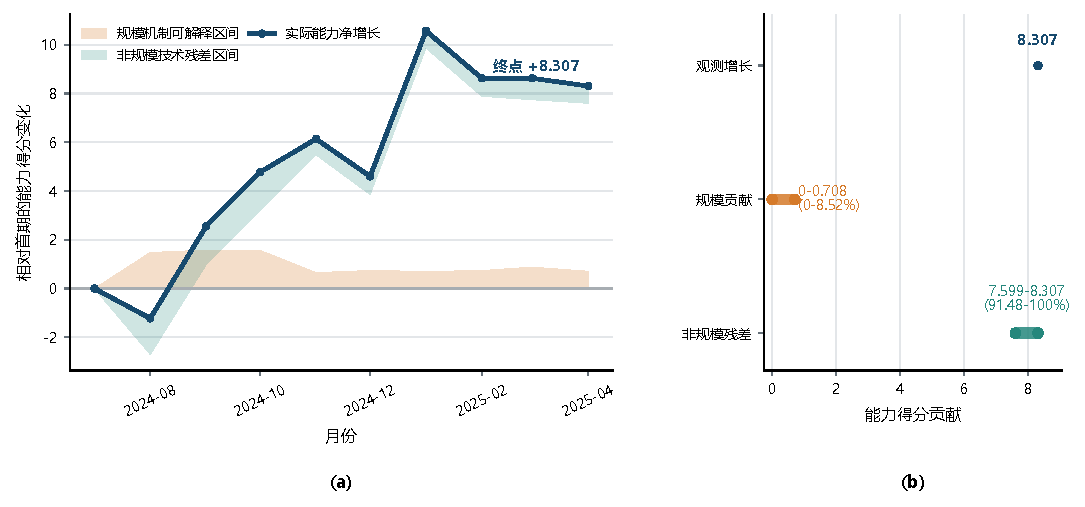
\includegraphics[width=0.92\textwidth,height=0.28\textheight,keepaspectratio]{figures/fig7_5_contribution_identification.pdf}
    \caption{能力增长的动态贡献分解与终点部分识别集合}
    \label{fig:q4-contribution}
\end{figure}

图~\ref{fig:q4-contribution}a进一步给出逐月识别路径。深色曲线为观测能力相对起点的净变化；橙色带表示规模机制可解释区间$[0,\Delta B_t^{(1)}]$；青色带表示由此反推的非规模综合项$[\Delta F_t-\Delta B_t^{(1)},\Delta F_t]$。2024年7月的短暂负值来自滚动窗口样本更替，此后观测能力持续上升。规模上界随算力前沿波动，最高约1.576分，期末收敛至0.708分；非规模综合项则随观测增长逐步累积，并在绝大多数月份承担主要变化。图~\ref{fig:q4-contribution}b报告期末识别集合，从动态路径与终点结构两个层面呈现同一分解结果。

为检验识别集合上端点对样本构成的敏感性，进一步分层重采样能力窗口、算力窗口和C6两层样本，并切换Q3三种成本形式，共实施1000次Bootstrap。表~\ref{tab:q4-contribution-stability}区分固定样本识别集合与上端点的重采样稳定性，后者不构成贡献率的置信区间。970次重采样产生有限份额；30次因能力净增长非正而比值不定义，24个有限上界超过100\%，均予以保留。有限上界中位数为12.73\%，97.5\%分位为85.34\%；上界低于10\%、25\%、50\%的比例分别为42.5\%、70.4\%、88.4\%。这表明“规模上界低于一半”在多数重采样中成立，而“规模上界低于10\%”的稳定性相对有限。

\begin{table}[htbp]
\caption{历史贡献识别集合及其上端点稳定性}
\label{tab:q4-contribution-stability}
\CompactTableSetup
\begin{tabularx}{0.90\textwidth}{@{}L C{2.55cm}Y@{}}
\toprule
证据层次 & 数值结果 & 统计含义\\
\midrule
观测能力净增长 & 8.307分 & 不依赖贡献分解假设的历史事实\\
固定样本规模贡献 & 0--0.708分；0--8.52\% & 共同支持边界下的部分识别集合\\
固定样本非规模贡献 & 7.599--8.307分；91.48\%--100\% & 与规模贡献互补的锚定残差集合\\
上端点Bootstrap中位数 & 12.73\% & 识别集合上端点的重采样中心\\
上端点Bootstrap高分位 & 97.5\%分位为85.34\% & 极端样本构成下的尾部敏感性\\
阈值稳定性 & 42.5\% / 70.4\% / \newline 88.4\% & 上端点低于10\%/25\%/50\%的比例\\
有效性审计 & 970有限；30未定义；24超过100\% & 未删除不利或极端结果\\
\bottomrule
\end{tabularx}
\TableNote[0.90\textwidth]{注：Bootstrap考察识别集合上端点的稳定性，不应解释为规模贡献率的置信区间。}
\end{table}

作为独立方向核验，C1--C4有128条可靠实体匹配，其中49条同时具备compute与能力得分，$\log_{10}$compute 与能力的Spearman相关为0.578，$p=1.35\times10^{-5}$。该结果支持规模作用方向为正，但不能消除发布时点、架构和数据质量的混杂，故不用于估计贡献率。由此获得了支持边界约束下的历史部分识别路径；下一节沿用同一状态方程，将算力路径与非规模状态共同推进至未来。

\subsection{算力放缓下的能力前沿预测}

历史分解确定了规模项与非规模状态项的接口，预测阶段不再引入独立的时间序列结构，而是沿用同一状态方程推进两条路径。本节先给出算力平台与技术漂移的情景设定，再报告条件模拟、不确定性来源及滚动起点回测。

\subsubsection{算力平台--技术漂移的双状态演化}

历史残差由$T_t=F_t-F_{t_0}-[B(C_t)-B(C_{t_0})]$锚定。对其采用带漂移随机游走$T_{t+1}=T_t+b+\eta_t$，其中$b$用Theil--Sen稳健斜率估计\cite{sen1968}，得到每月1.191分；创新标准差为2.663分。该漂移描述短期非规模综合项的延续速度，不解释为某项技术的因果效应。算力主情景令未来$\log_{10}C$增速为0；无放缓反事实则延续早期每月0.0812的增速。

将两种状态代回统一方程，$h$个月后的前沿为
\begin{equation}
F_{t+h}=F_t+\bigl\{B(C_{t+h})-B(C_t)\bigr\}
+bh+\sum_{j=1}^{h}\eta_{t+j}
.
\label{eq:q4-forecast}
\end{equation}
式~\eqref{eq:q4-forecast}不是独立的时间序列模型：第一项承接现实能力，第二项仍由问题三机制和桥接决定，后两项延续式~\eqref{eq:q4-state}中的同一非规模状态。因而历史解释、反事实和预测不会因更换模型而失去可比性。

\subsubsection{历史--预测统一的能力前沿推演}

表~\ref{tab:q4-scenarios}给出算力路径与技术漂移的$2\times2$有限情景。主情景“算力平台+当前漂移”的12个月点预测为53.358。保持技术漂移不变、将算力改为无放缓，只提高1.127分；保持算力平台、将技术漂移减半，则降低7.148分。由此，当前支持边界下的中期预测主要受非规模技术路径假设影响，而不是算力路径的细微差别。

\begin{table}[htbp]
\caption{12个月能力前沿的算力--技术情景矩阵}
\label{tab:q4-scenarios}
\CompactTableSetup
\begin{tabularx}{0.84\textwidth}{@{}L L C{1.75cm}C{1.75cm}@{}}
\toprule
算力路径 & 非规模技术路径 & 预测前沿 & 相对主情景\\
\midrule
平台（主情景） & 当前Theil--Sen漂移 & \textbf{53.358} & 0\\
平台 & 半漂移 & 46.210 & $-7.148$\\
延续早期增速 & 当前Theil--Sen漂移 & 54.484 & $+1.127$\\
延续早期增速 & 半漂移 & 47.336 & $-6.021$\\
\bottomrule
\end{tabularx}
\TableNote[0.84\textwidth]{注：情景矩阵用于结构反事实，不赋予四种路径主观发生概率。}
\end{table}

条件模拟共2000次，逐次传播七类不确定性：终点能力窗口、模型族依赖、终点算力窗口、Q3成本形式、High/Medium桥接样本、支持边界后斜率，以及技术漂移和随机游走创新。图~\ref{fig:q4-forecast}以50\%、80\%、95\%三层色带连接起点与12/24月模拟端点。12个月模拟中位数为51.203，95\%条件区间为$[24.220,78.336]$；该区间刻画给定情景与重采样规则下的不确定性传播，不属于频率学置信区间。

\begin{figure}[htbp]
    \centering
    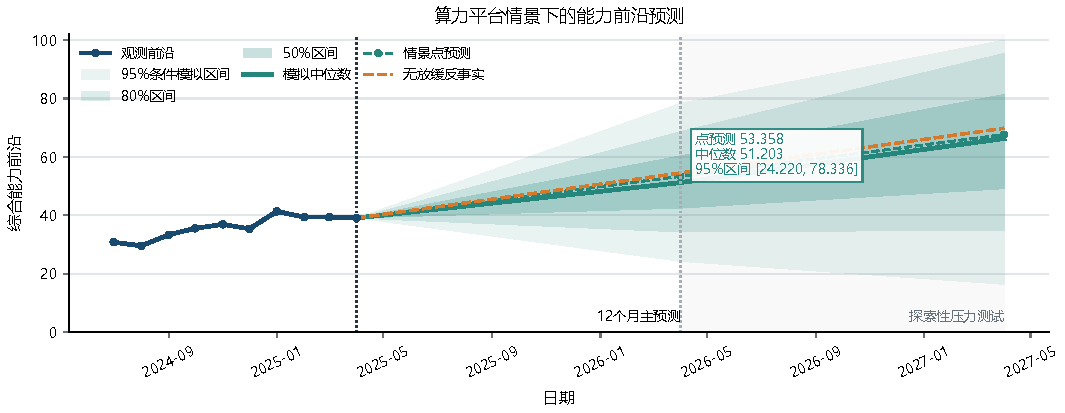
\includegraphics[width=0.92\textwidth,height=0.27\textheight,keepaspectratio]{figures/fig7_6_capability_forecast.pdf}
    \caption{算力平台情景下开放权重模型能力前沿的条件预测}
    \label{fig:q4-forecast}
\end{figure}

24个月点预测为67.654，中位数66.296，95\%区间为$[16.336,100]$，上端触及量表边界。该结果表明现有证据在这一期限已不足以约束分布上尾，并不意味着能力必然达到量表上限。因此，12个月作为主预测期限，13--24个月仅作为压力测试，并在图中以灰色背景降低其证据等级。

\subsubsection{预测不确定性的来源归因}

条件区间的宽度不仅取决于随机游走创新，还受到能力样本、模型族结构和跨问题机制接口的共同影响。为识别主要来源，本文采用单因素方差缩减实验：在保持其余来源随机的条件下，将第$j$类不确定性固定为主设定值，并在同一模拟抽样批次下重新估计12个月预测。定义
\begin{equation}
R_j
=
1-\frac{\operatorname{Var}(F_{12}\mid U_j=\bar U_j)}
        {\operatorname{Var}(F_{12})}.
\label{eq:q4-uncertainty-reduction}
\end{equation}
$R_j$衡量固定单一来源后总方差的相对缩减。由于各来源存在非线性交互且预测值受0--100边界截断，该指标不具可加性，也不解释为Sobol指数。

完整模拟的12个月预测方差为187.300，对应标准差13.686。图~\ref{fig:q4-uncertainty}显示，固定技术漂移与创新后方差缩减93.79\%，显著高于模型族依赖的3.71\%和能力窗口抽样的1.72\%；支持域外斜率、算力前沿、Q3成本形式及桥接样本的单因素影响均接近0。Q3成本形式和桥接样本出现$-0.00\%$与$-0.01\%$的微小负值，源于非线性交互、量表截断及有限模拟误差，不表示其产生“负不确定性”。因此，预测区间的主要宽度来自非规模技术状态的未来延续，而非对算力路径的局部扰动；该发现也与情景矩阵中技术漂移变化造成更大预测位移相互印证。

\begin{figure}[htbp]
    \centering
    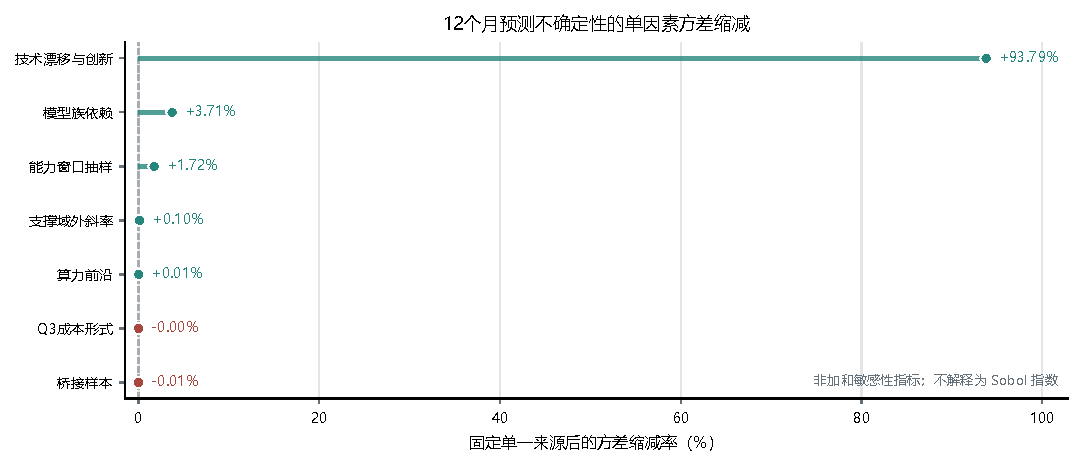
\includegraphics[width=0.92\textwidth,height=0.27\textheight,keepaspectratio]{figures/fig7_7_uncertainty_attribution.pdf}
    \caption{12个月能力预测不确定性的单因素方差缩减}
    \label{fig:q4-uncertainty}
\end{figure}

\subsubsection{条件模拟传播与滚动起点回测}

采用rolling-origin方式，在每个历史起点只使用此前信息预测未来1、2、3个月，共得到每种方法12个预测。对照包括最后值保持和直接对$F_t$作Theil--Sen外推。图~\ref{fig:q4-backtest}a显示统一模型95\%条件区间覆盖率为91.7\%，各期限覆盖率为80\%、100\%、100\%；平均宽度随期限由10.237增至16.438，符合随机游走不确定性随时间累积的方向。

\begin{figure}[htbp]
    \centering
    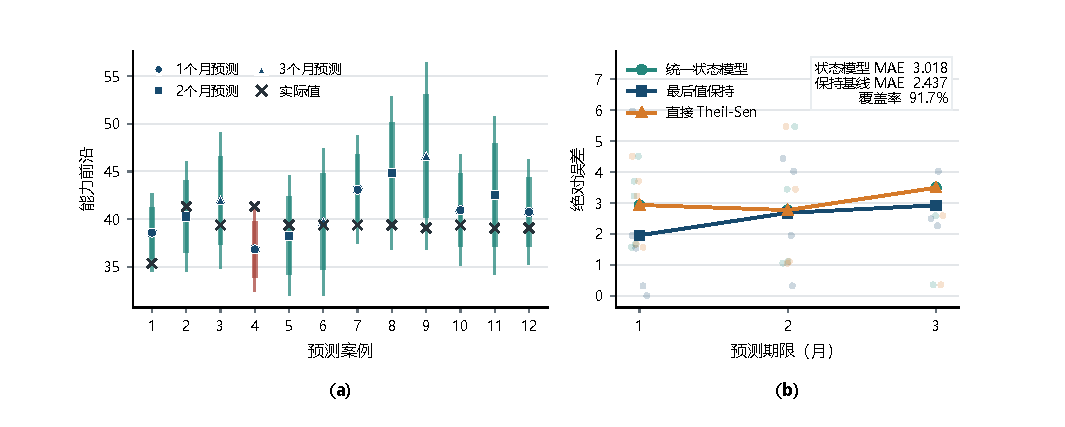
\includegraphics[width=0.92\textwidth,height=0.27\textheight,keepaspectratio]{figures/fig7_8_forecast_backtest.pdf}
    \caption{能力前沿预测的滚动起点回测与简单基线比较}
    \label{fig:q4-backtest}
\end{figure}

\begin{table}[htbp]
\caption{统一状态模型与简单基线的滚动起点回测}
\label{tab:q4-backtest}
\CompactTableSetup
\begin{tabularx}{0.88\textwidth}{@{}L C{1.40cm}C{1.40cm}C{1.40cm}C{1.55cm}@{}}
\toprule
方法或区间指标 & 1个月（$n=5$） & 2个月（$n=4$） & 3个月（$n=3$） & 总体（$n=12$）\\
\midrule
统一状态模型MAE & 2.934 & 2.767 & 3.493 & 3.018\\
最后值保持MAE & \textbf{1.952} & \textbf{2.678} & \textbf{2.923} & \textbf{2.437}\\
直接Theil--Sen MAE & 2.934 & 2.767 & 3.493 & 3.018\\
\midrule
共同95\%覆盖率 & 80.0\% & 100.0\% & 100.0\% & 91.7\%\\
共同平均区间宽度 & 10.237 & 14.212 & 16.438 & 13.112\\
\bottomrule
\end{tabularx}
\TableNote[0.88\textwidth]{注：三种方法共用历史残差尺度，故区间指标相同；加粗值表示同期限最小MAE。}
\end{table}

图~\ref{fig:q4-backtest}b与表~\ref{tab:q4-backtest}表明，最后值保持在三个期限均取得最小MAE，统一状态模型的短期点预测精度未优于简单基线。直接Theil--Sen与统一模型在本回测窗口内完全重合，原因在于各训练折的算力机制项在域外饱和边界下为0；在无放缓算力反事实中，两者不再等价。由于三种方法共享同一残差尺度，其区间覆盖率与平均宽度相同，不能据此判断统一状态模型具有更优的概率校准。

点预测精度与结构反事实效用属于不同评价维度。对于一至三个月的短期点预测，最后值保持具有更低误差；对于算力增速继续放缓如何影响能力前沿这一结构性问题，统一状态模型能够分离算力路径与非规模技术路径，因而具有简单预测基线不具备的反事实解释功能。

\paragraph{本问小结}
问题四得到四项主要结论。第一，开放权重chat/finetuned模型的能力前沿提高8.307分，指标信度、多口径和模型族平衡检验均支持总体上升方向，但GPQA并未同步改善。第二，来源校准单调桥接显式处理了跨来源水平偏差，绝对映射误差仍作为不确定性进入后续分析。第三，现实算力与映射Loss均超出共同支持域，规模贡献仅能部分识别；固定样本识别集合为0\%--8.52\%，不支持唯一的点分解比例。第四，算力平台情景下的12个月点预测为53.358，区间宽度主要由非规模技术状态的延续决定，且短期点预测精度未优于保持基线。综上，本文形成了\textbf{支持边界感知、来源截距不变、历史分解与情景预测统一}的能力前沿状态框架，使“能力如何度量、Loss如何映射、历史增长如何识别及算力放缓后如何演化”构成闭合证据链。
